\documentclass [handout]{beamer}
\usepackage{pgfpages}
\usepackage{listings}
\usepackage{verbatim}
\usetheme[secheader]{Madrid}
\useoutertheme{infolines}
\usepackage[utf8]{inputenc}
\usepackage{graphicx}
\usetheme[secheader]{Madrid}
\useoutertheme{infolines}
\date{ 23 octobre 2014 }
\definecolor{LHCblue}{HTML}{058013}
\usecolortheme[named=LHCblue]{structure}
\title{Qt-Designer}
\author{Jihen Fourati - Hadil Fajraoui}
\institute[UM2]
{
  Département informatique
  Université de Montpellier 2
}
\begin{document}

\begin{frame}
  \titlepage 
\end{frame}
\section{Sommaire}
\begin {frame}[fragile]{Sommaire}
 \begin{enumerate}
  \item Introduction à la notion de  Qt-designer 
  \item Dérivation / Génération de code
  \item Compilation
  \item Les signaux et les slots
  \item Conclusion
  \item Sources
 \end{enumerate}
\end{frame}

\section{Introduction à la notion de  Qt-designer}
\begin{frame}[fragile]{Qu'est ce que Qt-Designer ?}
 \begin{itemize} [<+-|alert@+>]
  \item Outil de développement d'interface graphique.
  \item Concepteur de fenêtre.
  \item Complément de Qt-Creator: fait parti du Qt Frameworks
 \end{itemize}
\end{frame}
\begin{frame}[fragile]{Un peu d'histoire}
 \begin{itemize} [<+-|alert@+>]
  \item 1994: Qt  - Qt est une bibliothèque  multiplateforme développé en C++, créé en 1994.
  \item 1995: Qt1 - Première version publique de Qt
  \item 2000: Qt2 -La seconde version majeure de Qt 
  \item 2001:Qt3 - Nouvelle version apporte un meilleur support de l'internationalisation,de l'Unicode.
  \item 2005: Qt4 - Première version de Qt séparée en modules \\
  Apparition de Qt Designer
 \end{itemize}
\end{frame}
\begin{frame}[fragile]{A quoi sert Qt-designer ?}
C'est un outil de création d'interface graphique.
\pause
 \begin{itemize} [<+-|alert@+>]
  \item Constructeur de GUI pour Qt
  \item Ce n'est pas un IDE 
  \item Ne produit aucun code  
  \item Gratuit 
 \end{itemize}
\end{frame}
\section{Analyse de la fenêtre de Qt Designer }
\begin{frame}[fragile]{L'interface}
 \begin{center}
  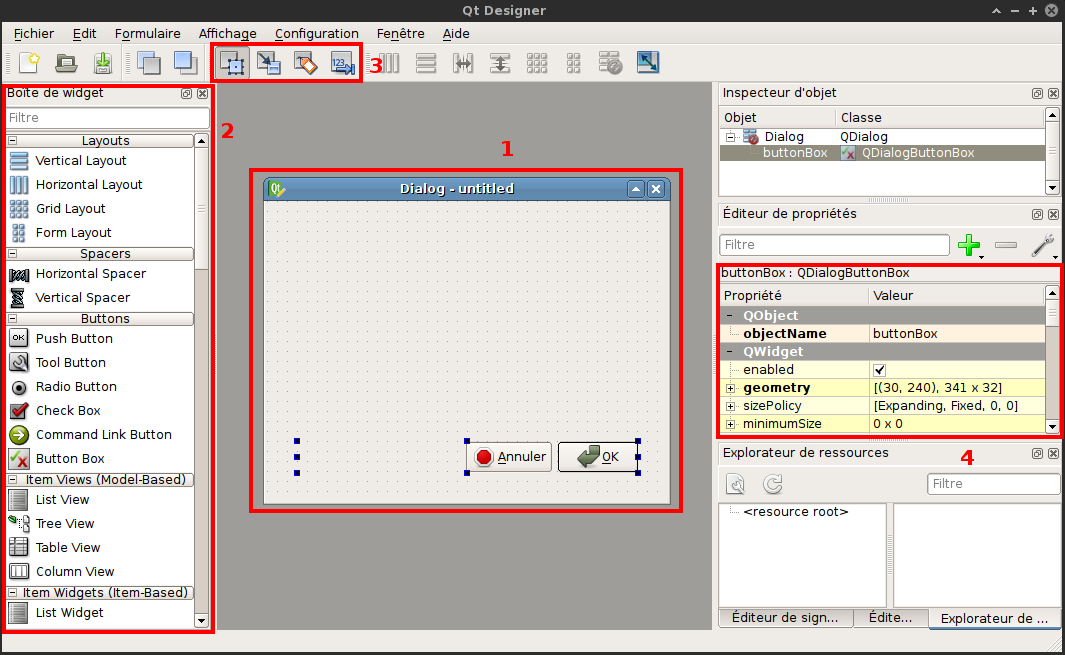
\includegraphics[scale=0.25]{InterfaceGenerale.png}
 \end{center}
\end{frame}

\begin{frame}[fragile]{Les buttons}
 \begin{center}
  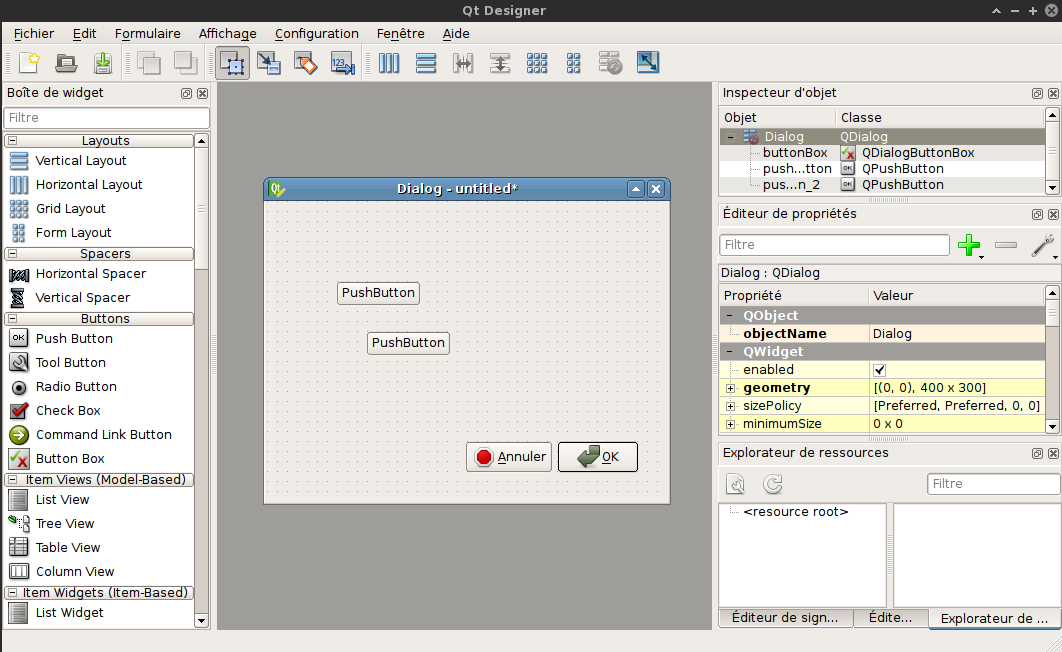
\includegraphics[scale=0.25]{Sanslayout.png}
 \end{center}
\end{frame}

\begin{frame}[fragile]{ Layouts}
 \begin{center}
  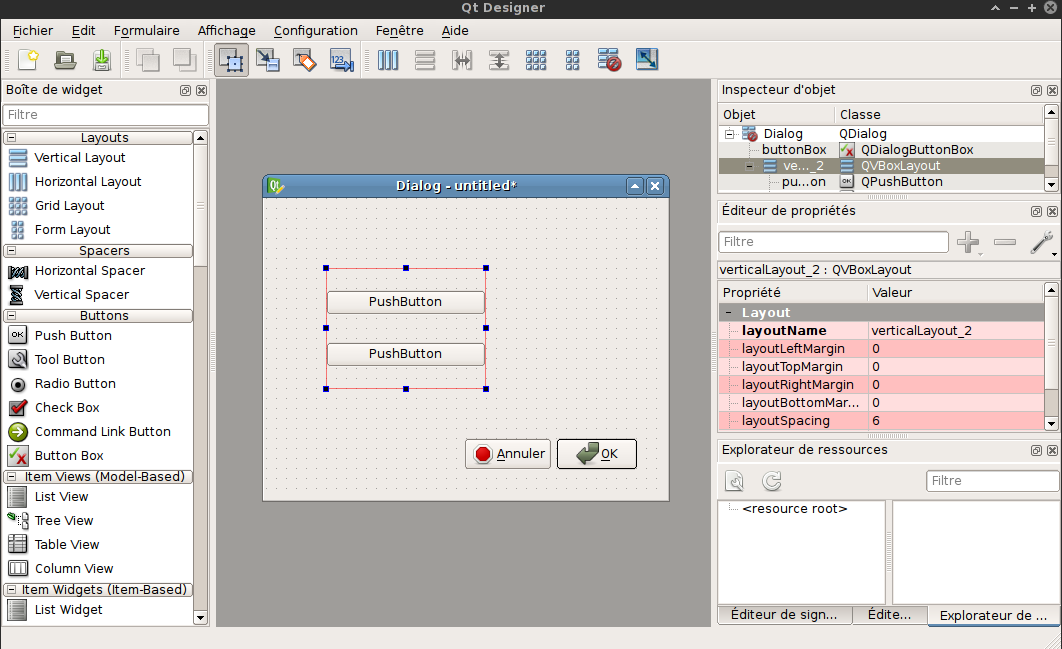
\includegraphics[scale=0.25]{Layout.png}
 \end{center}
\end{frame}

\begin{frame}[fragile]{ Spacers}
 \begin{center}
  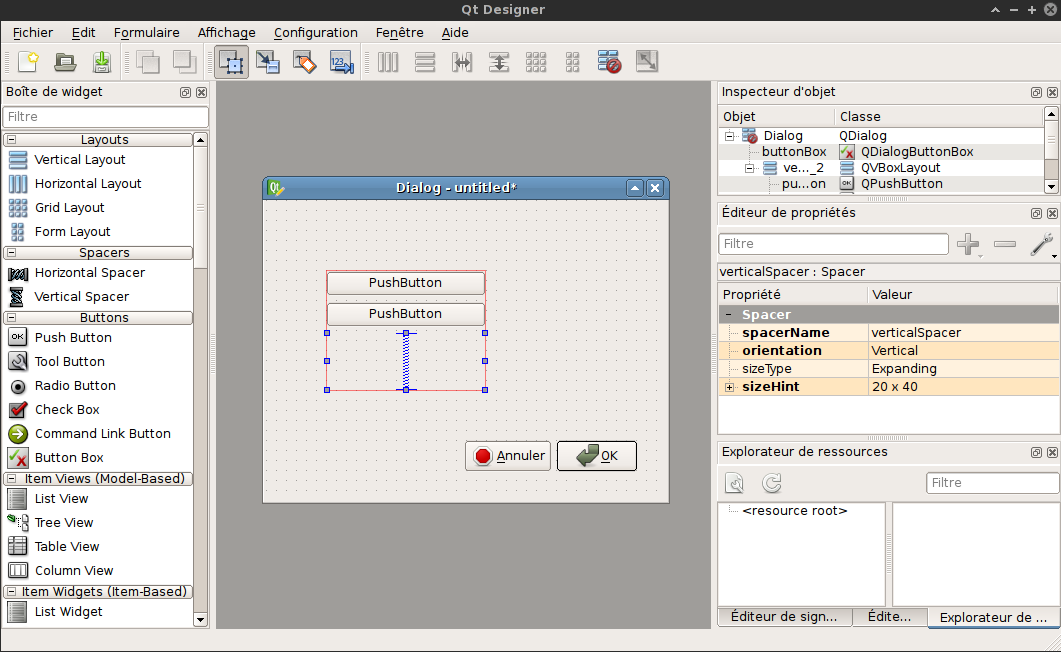
\includegraphics[scale=0.25]{Layoutavecspacer.png}
 \end{center}
\end{frame}

\begin{frame}[fragile]{Configurer les signaux et les slots}
 \begin{center}
  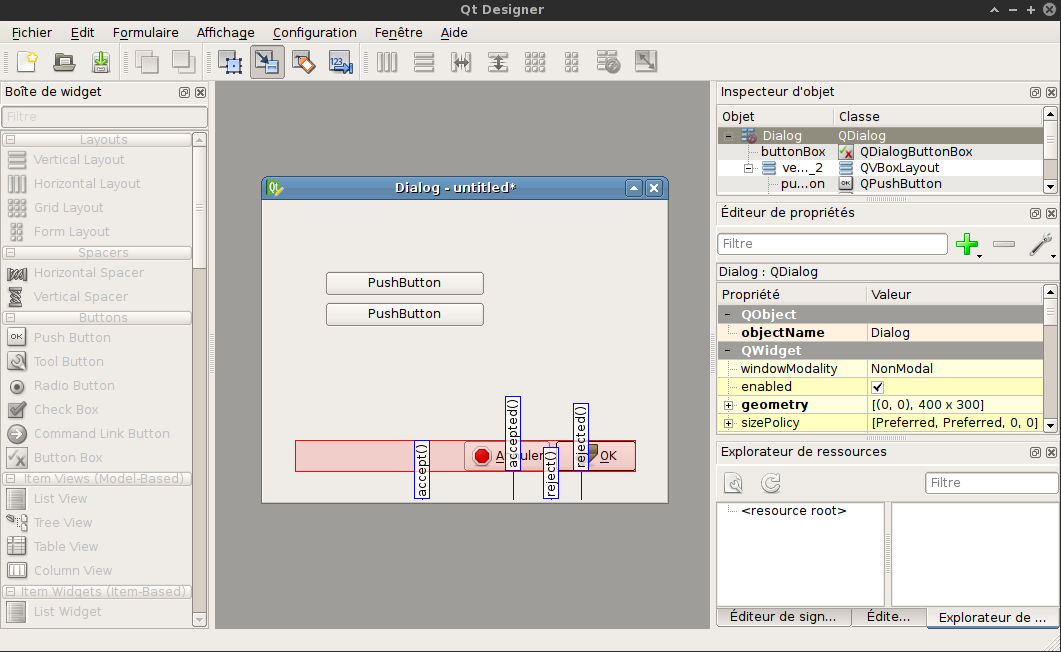
\includegraphics[scale=0.25]{Signaux1.png}
 \end{center}
\end{frame}

\begin{frame}[fragile]{Configurer les signaux et les slots}
 \begin{center}
  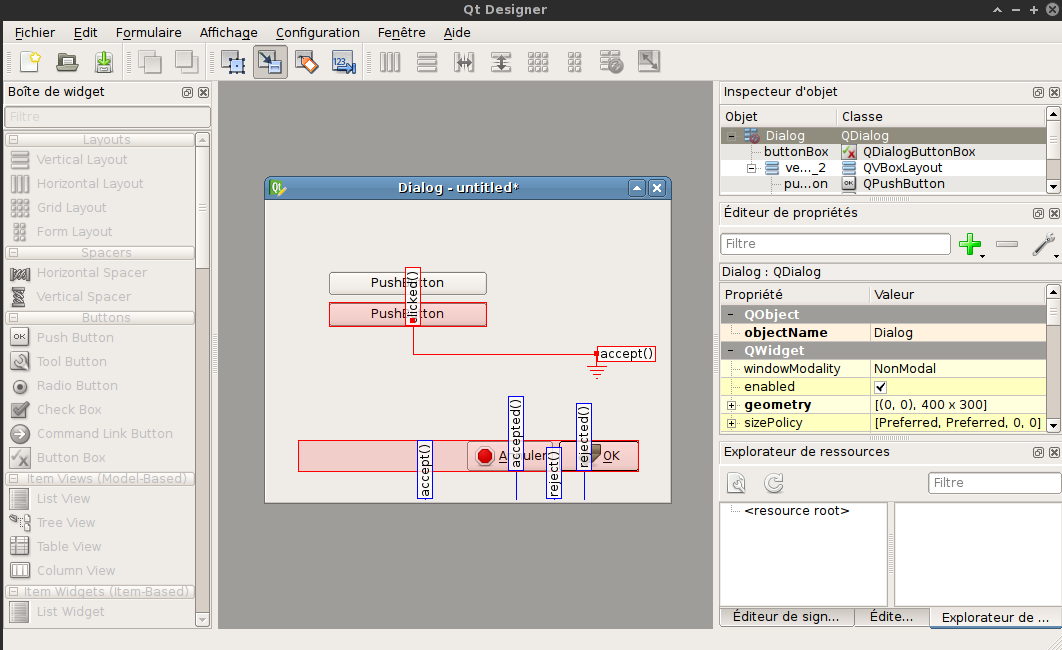
\includegraphics[scale=0.25]{Signaux2.png}
 \end{center}
\end{frame}

\begin{frame}[fragile]{Configurer les signaux et les slots}
 \begin{center}
  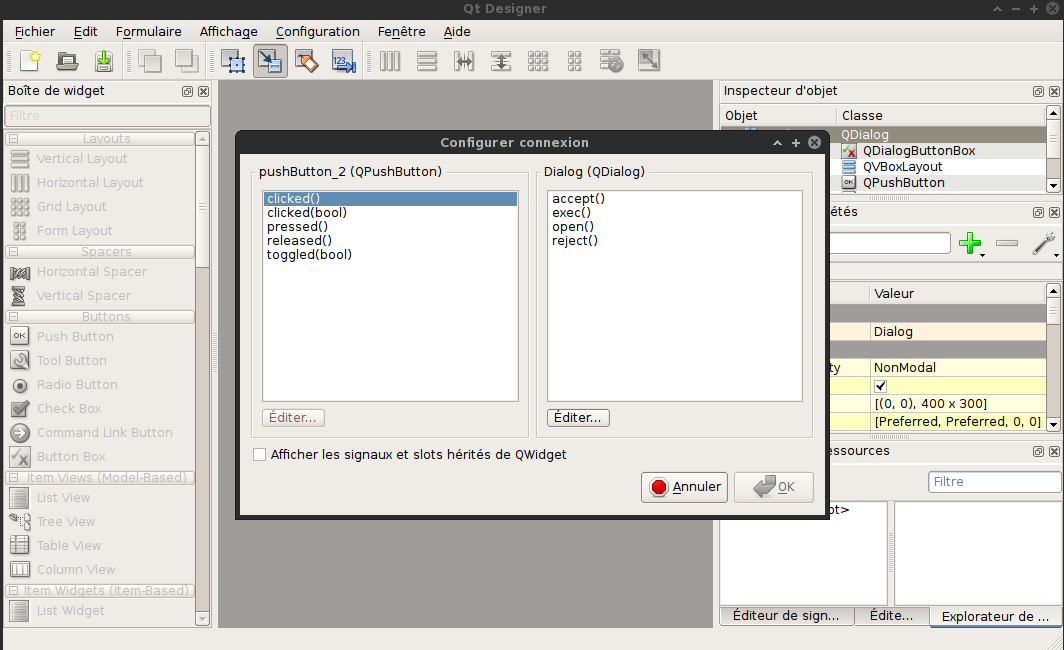
\includegraphics[scale=0.25]{Signaux3.png}
 \end{center}
\end{frame}
\section{Dérivation / Génération de code}
\begin{frame}[fragile]{Le principe de la génération du code source}
\begin{center}
  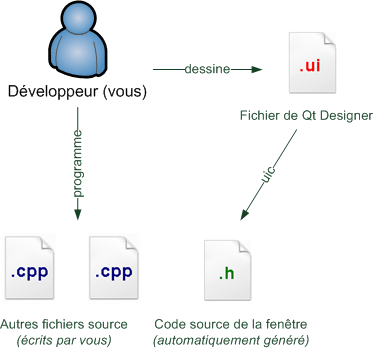
\includegraphics[scale=0.35]{ui.jpg}
 \end{center}
\begin{block}{}
Vous dessinez la fenêtre avec Qt Designer qui produit un fichier .ui.
Ce fichier est transformé automatiquement en code source par le petit programme en ligne de commande uic. Celui-ci génèrera un fichier ui\_nomDeVotreFenetre.h. Qt met tout le code dans le fichier .h    
\end{block}
\end{frame}
\begin{frame}[fragile]{Dérivation / Génération de code}
\begin{center}
  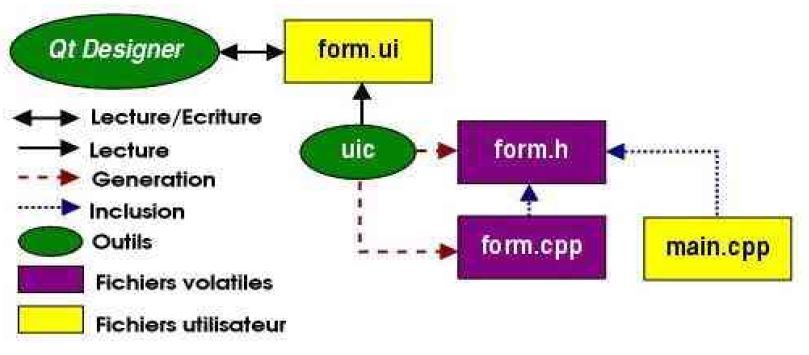
\includegraphics[scale=0.35]{1.jpg}
 \end{center}
 \begin{block}{}
Toute modification apportée au code généré automatiquement à partir de
l'interface graphique (fichier .ui) sera perdu à chaque recompilation      
    \end{block}
\end{frame}
\begin{frame} {Dérivation / Génération de code}
\begin{center}
  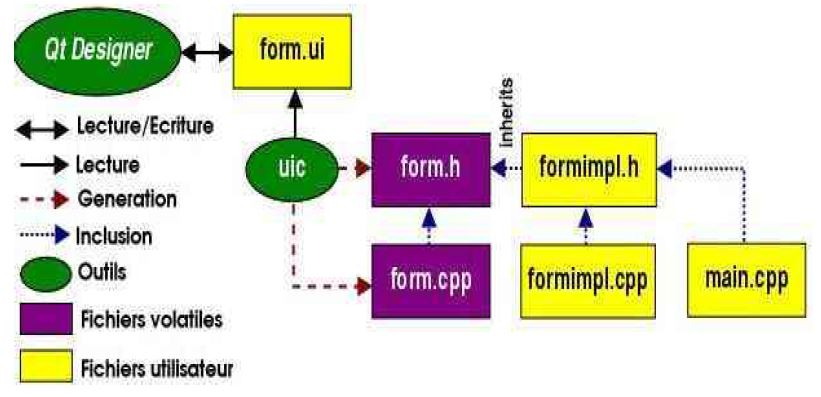
\includegraphics[scale=0.35]{3.jpg}
 \end{center}
 \begin{block}{}
Pour éviter ce désagrément, il faudra écrire une classe qui dérive de la classe
principale de votre interface et y implémenter vos slots et signaux.     
 \end{block}
 \end{frame} 

\begin{frame}[fragile]{Dérivation / Génération de code}
\begin{center}
  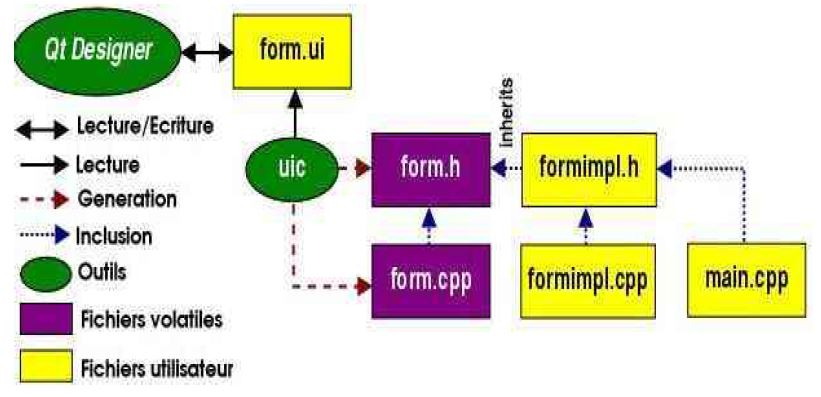
\includegraphics[scale=0.35]{3.jpg}
 \end{center}
 \begin{block}{}
Une autre méthode consiste à généré du code cpp embarqué dans l'interface
graphique. Cette méthode est à déconseiller car elle disparaître dans les
prochaines versions de QT.     
    \end{block}
\end{frame} 

\section{Compilation}
 \begin {frame}{} 
Le .h correspondant au .ui n'est pas éditable par défault dans Qt Creator, en effet, celui ci est généré au moment de la compilation (et donc toute modification est écrasée).\newline \newline

Dans le Makefile, on a :\newline \newline

ui\_mainwindow.h: mainwindow.ui\newline
/usr/bin/uic mainwindow.ui -o ui\_mainwindow.h
\end {frame}
\section{Les signaux et les slots}
\begin{frame}{Le principe des signaux et slots}{}
\begin{center}
\item{ Voici un schéma qui montre ce qu'un objet pouvait contenir avant Qt, ainsi que ce qu'il peut contenir maintenant qu'on utilise Qt (figure suivante).}
  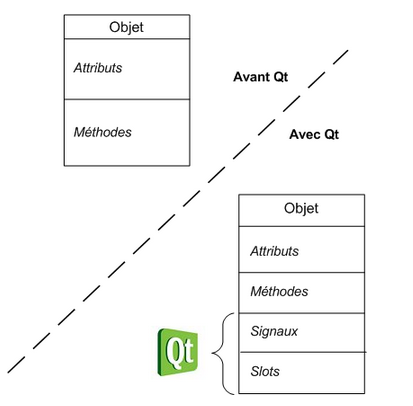
\includegraphics[scale=0.30]{Capture1.jpg}
 \end{center}
    \pause
    
Exemple connexion signaux et  slot:
    \begin{center}
    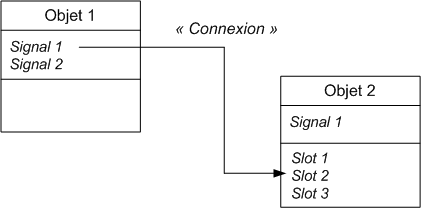
\includegraphics[scale=0.30]{sc.png}
    \end{center}
   
\end{frame}
\section{Conclusion}
\begin{frame}{Conclusion}
    \begin{itemize}
    \item{Qt Designer est un programme qui permet de construire rapidement ses fenêtres à la souris. Il nous évite l'écriture de nombreuses lignes de code.}
    \item{Qt Designer est intégré à Qt Creator mais existe aussi sous forme de programme externe. Il est conseillé de l'utiliser dans Qt Creator car le fonctionnement est plus simple.}
    \item{Qt Designer crée automatiquement un fichier de code qui place les widgets sur la fenêtre. On travaille ensuite sur une classe qui hérite de ce code pour adapter la fenêtre à nos besoins.}
    \end{itemize}
\end{frame}
\section{Sources}
\begin {frame}[fragile]{Sources}
 \begin{enumerate}
  \item http://www.wikipedia.org/
  \item http://www.stackoverflow.com/
  \item http://www.siteduzero.com/
 \end{enumerate}
\end{frame}
\section{DOCUMENTATION (HTTP//WWW.DOC.QT.NOKIA.COM/)}
\begin{frame}[fragile]{DOCUMENTATION (HTTP//WWW.DOC.QT.NOKIA.COM/)}
 \begin {itemize}
\item Tutoriel : http://doc.trolltech.com/4.7/tutorials.html
  \item qmake (http://doc.trolltech.com/4.7/qmaketutorial.
html) ;
  \item Qt Designer (http://doc.trolltech.com/4.7/designermanual.
html) ;
  \item Qt Creator (http://doc.qt.nokia.com/qtcreator2.0/
index.html).
 \end{itemize}
\end{frame}
\section{DOCUMENTATION}
\begin{frame}[fragile]{DOCUMENTATION}
 \begin {itemize}
\item Quelques autres sources d'informations méritant le détour :
  \item Qt Centre : http://www.qtcentre.org/
  \item Qt Forum (en anglais) : http://www.qtforum.org/
  \item QtFr, un site français, http://www.qtfr.org/
  \item Qt Designer : http://qt.developpez.com/tutoriels/

 \end{itemize}
\end{frame}
\section{}
\begin{frame}{}
    \centering
    \textbf{Merci de votre attention}
\end{frame}


\end{document}
